\question
$\mathbf{p}=\left(\begin{array}{l}
2 \\
3
\end{array}\right) \quad \mathbf{q}=\left(\begin{array}{r}
-3 \\
2
\end{array}\right)$\\
\begin{parts}
\part 
On the unit grid below, draw and label vector $\mathbf{p}$.\\
\begin{center}
        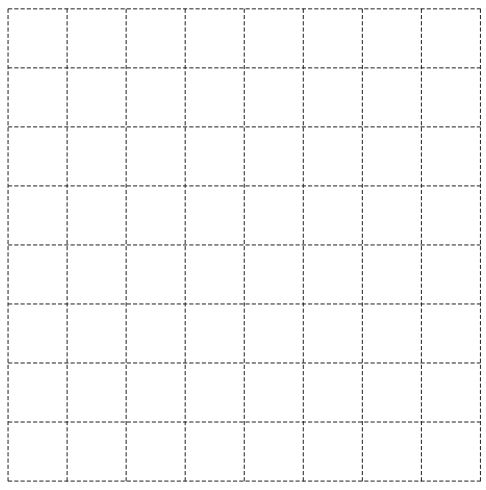
\includegraphics[scale=0.6]{Questions/quiz 16/images/6.JPG}
\end{center}
{\flushright{
\hfill           [1]}}
\\ 
\part On the unit grid below, draw and label vector $2q$.\\
\begin{center}
        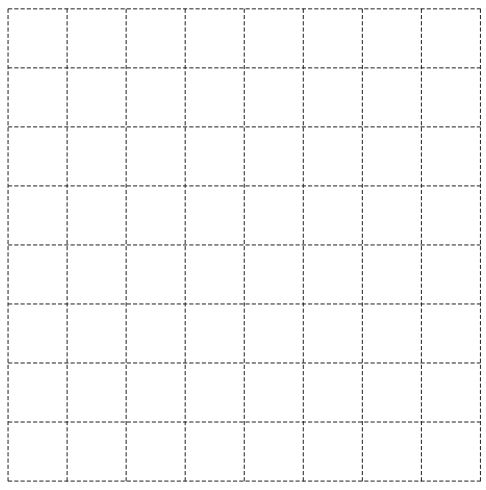
\includegraphics[scale=0.6]{Questions/quiz 16/images/6.JPG}
\end{center}
{\flushright{
\hfill           [1]}}\\
\part On the unit grid below, draw and label vector $p- q$.\\ 
\begin{center}
        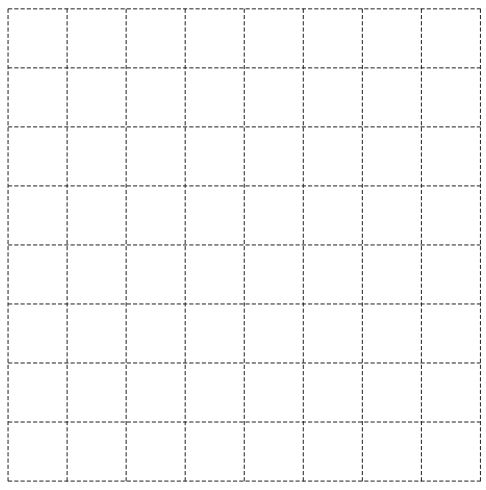
\includegraphics[scale=0.6]{Questions/quiz 16/images/6.JPG}
\end{center}
{\flushright{
\hfill           [2]}}
\end{parts}